\section{Система оценки эффектиивности алгоритмов шумоподавления}
\subsubsection{Изображения}
Для исследования были взяты изображения из открытой базы данных ImageNet, а так же из личной коллекции.  Была произведенна следующая классификация и для каждой классификации было взято по 20 изображений с разрешением в среднем $450 \times 450$:
\begin{itemize}
	\item Изображения людей
	\item Изображения архитектуры
	\item Изображения полученные при недостаточной освещенности
\end{itemize}
Данная классификация обусловлена распространенностью данных классов изображений и прикладных задачах в области обработки изображений. Фотографии людей используются как в повседневной жизни, так и во многих алгоритмах компьютерного зрения, таких как например распознавание лиц.

Не менее распространенны так же и изображения полученные при недостаточной освещенности, что приводит к низко контрастному изображению. Это мешает их анализу. Так же данные это актуально и для обычных пользователей фото и видеокамер, устройство которых все еще не позволяет достичь приемлимых результатов при съемке ночью. 

Последняя категория была выбрана в качестве примера, где  некоторые части изображения похожи друг на друга. Это может быть полезно в таких областях связанных с медициной, электроникой и астрономией. Где изображения, необходимы для последующей обработки имеют подобные свойства.

Для каждой категории было отобрано по 20 изображений. Ниже приведены примеры некоторых из них.

\begin{figure}[H]
	\begin{minipage}[H]{0.49\linewidth}
		\center{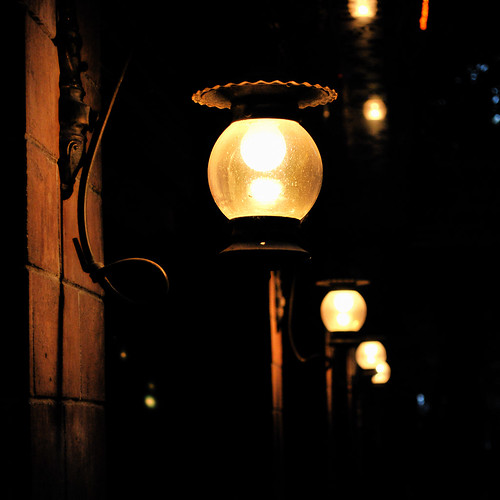
\includegraphics[scale=0.5]{imageNight} \\ а) Ночная съемка}
	\end{minipage}
	\begin{minipage}[H]{0.49\linewidth}
		\center{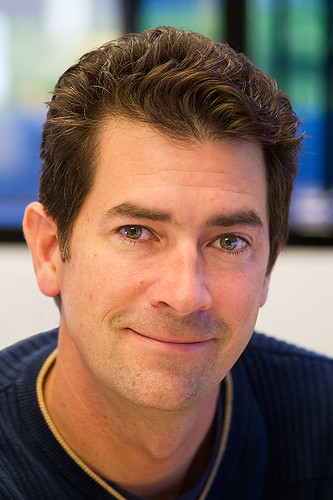
\includegraphics[scale=0.5]{imagePerson} \\ б) Человек}
	\end{minipage}
	\begin{center}
		\begin{minipage}[H]{0.49\linewidth}
			\center{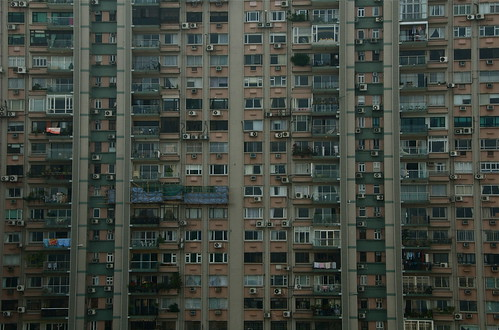
\includegraphics[scale=0.5]{imageArchitecture} \\ в) Архитектура}
		\end{minipage}
	\end{center}
	\caption{Примеры изображений различных категорий}
\end{figure}


\subsubsection{Видео}
Данные необходимые для исследования видео последовательность были взяты из открытой базы данных  YouTube-8M\cite{youtube8m}.


Было выбранно 10 видеопоследовательностей каждой категории, в среднем с разрешением $1920 \times 720$ и содержать примерно по $300$ кадров. Ниже приведены кадры из видео каждой категории.
\begin{figure}[H]
	\begin{minipage}[H]{0.49\linewidth}
		\center{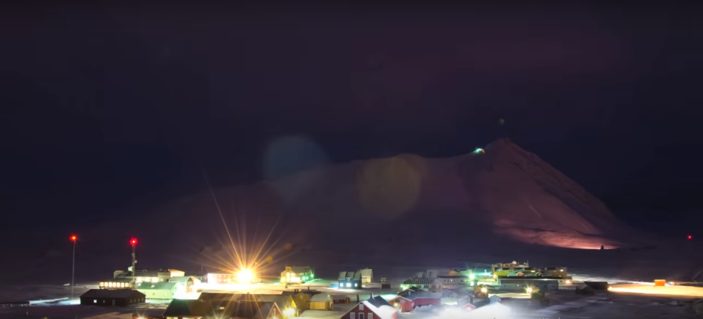
\includegraphics[trim={1.5cm 0cm 1.5cm 0cm},scale=1,clip]{videoNight} \\ а) Ночная съемка}
	\end{minipage}
	\begin{minipage}[H]{0.49\linewidth}
		\center{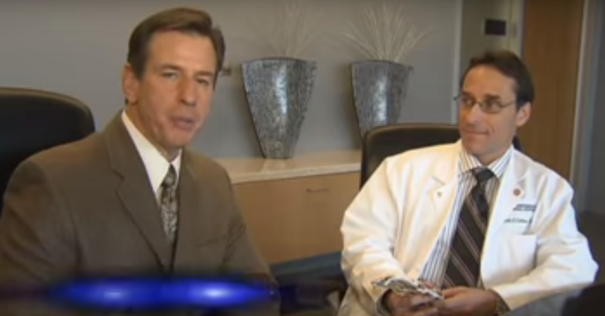
\includegraphics[trim={1.5cm 0cm 1.5cm 0cm},scale=1,clip]{videoPerson} \\ б) Человек}
	\end{minipage}
	\begin{center}
		\begin{minipage}[H]{0.49\linewidth}
			\center{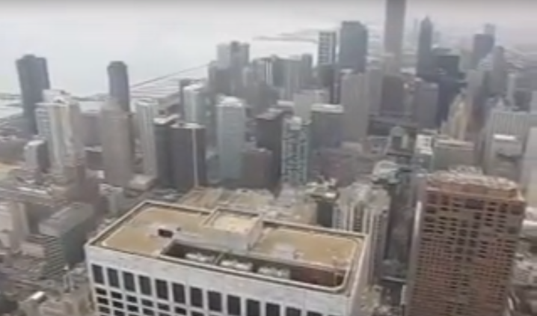
\includegraphics[]{videoArchitecture} \\ в) Архитектура}
		\end{minipage}
	\end{center}
	\caption{Примеры кадров видео различных категорий}
\end{figure}
\subsection{Схема программы}
Работу реализованной программы можно описать следующим образом. На вход программы подаются данные (видео или изображение). Далее накладывается гауссовский шум. После проводится шумоподавления различными алгоритмами с различными параметрами. В итоге выбирается алгоритм, которые показал наибольшие показатели PSNR и SSIM. 
\begin{figure}[H]
	\center{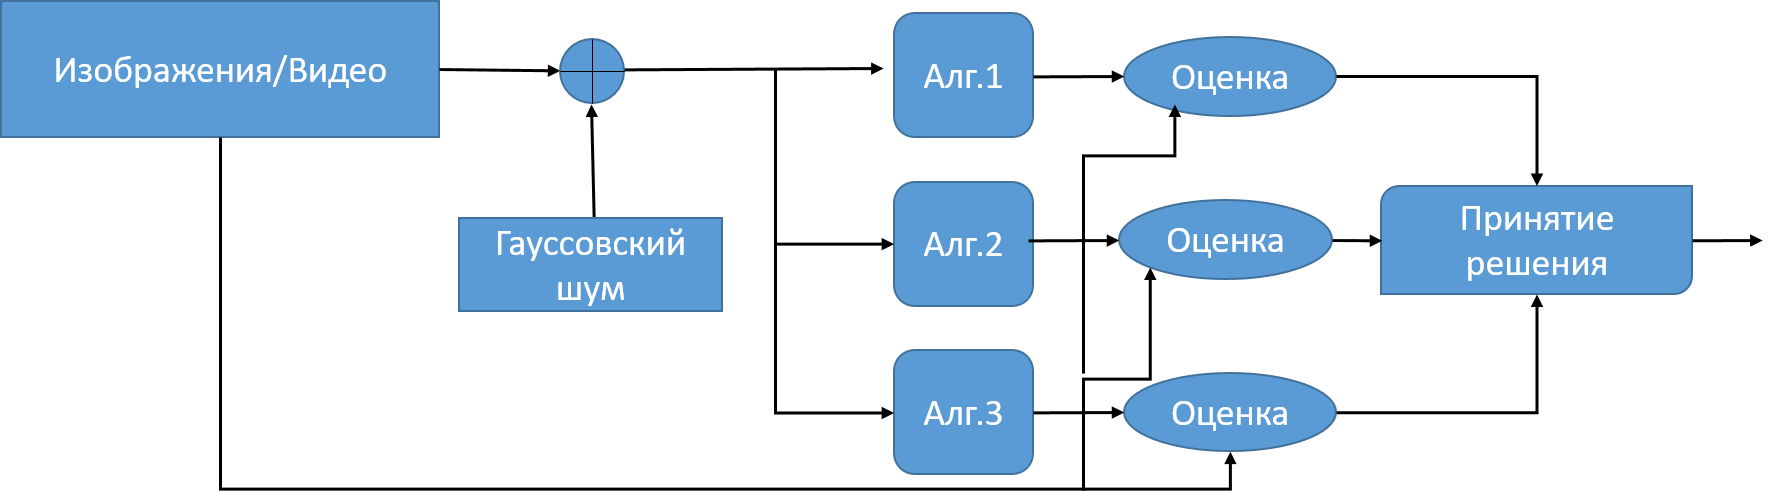
\includegraphics[scale=0.5]{circuitProgram}}
	\caption{Схема итоговой программы}
\end{figure}
\subsection{Критерии оценки эффективности алгоритмов}
\subsubsection{PSNR}\label{sec:PSNR}
Для оценки степени искажения изображений, используются различные методы. Самым популярным является PSNR(pick signal-noise-to-noise ratio). Он обозначает соотношение между максимумом возможного значения изображения и мощностью шума, который искажает данное изображение. Значения лежат в диапазоне от $(0, \infty)$, чем больше PSNR, тем изображение считается близки к оригиналу.
\begin{equation}\label{eq:PSNR}
PSNR = 10log_{10}(\frac{MAX_I^2}{MSE})
\end{equation}
где 
\begin{itemize}
	\item $MAX_I$ - максимально возможное значения пикселя
	\item $MSE = \frac{1}{nm}\sum_{i=0}^{n}\sum_{j=0}^{m}(x_{i,j} - y_{i,j})^2$ - средний квадрат ошибки между оригинальным изображением x и искаженным y.
	\item m,n - высота и ширина изображения
\end{itemize}
PSNR имеет как ряд преимуществ так и некоторые недостатки. К преимуществам относят быстроту и легкость вычисления. К недостаткам: для вычисления необходимо иметь исходную и преобразованную картинку, при этом не может быть точно известно, что  оригинальная картинка не имела искажений, так же в ряде случаев PSNR плохо коррелирует с субъективными мерами оценки  качества. Т.е. высокие значения PSNR не всегда обеспечиваются лучшим качеством картинки с визуальной точки зрения.
\subsection{SSIM}
Из-за несовершенств метрики PSNR разрабатывались все новые и новые методики. Одной из который является SSIM (Structural SIMilarity). Отличительной особенностью метода, является то, что метод учитывает «восприятие ошибки» благодаря учёту структурного изменения информации. Идея заключается в том, что пиксели имеют сильную взаимосвязь, особенно когда они близки пространственно. Данные зависимости несут важную информацию о структуре объектов и о сцене в целом\cite{ssim}.
\begin{equation}\label{eq:SSIM}
SSIM = \frac{(2\mu_x\mu_y+c_1)(2\sigma_{x,y}+c_2)}{(\mu_x^2+\mu_y^2+c_1)(\sigma_x^2+\sigma_y^2+c_2))}
\end{equation}
где
\begin{itemize}
	\item $\mu_x$ - среднее х
	\item $\mu_y$ - среднее y
	\item $\sigma_x^2$ - дисперсия x
	\item $\sigma_y^2$ - дисперсия y
	\item $\sigma_{x,y}^2$ - ковариация x и \item $c_1=(k_1L)^2, c_2=(k_2L)^2$ - две переменных
	\item $L$ - динамический диапазон(максимальное значение пикселя)  
	\item $k_1=0.01, k_2=0.03$ - константы
\end{itemize}
Формула \ref{eq:SSIM} указана только для яркостной компоненты. Значения находятся в отрезке $(-1,1)$, если значение +1, то изображение наиболее похожи. При полном несоответствии -1. Так же данная метрика зависит от размера окна, обычно размер берется $8\times8$.\

\subsubsection{Выбор оптимального алгоритма}
На основе критериев эффективности алгоритмов приведенных выше был предложен следующий метод оценки оптимального алгоритма. Для каждой категории изображений производятся испытания всех реализованных алгоритмов с различными параметрами. Алгоритмы, которые показали максимальные значения SSIM и PSNR для большего количества изображений объявляются оптимальными.

\subsection{Выводы по разделу}
Развитие критериев оценивания схожести двух изображений продолжается и по сей день. Охватить их в полном объеме не получится, поэтому для дипломной работы были выбраны наиболее популярные метрики, хоть они и обладают некоторым недостатком. А именно, для них необходимо иметь не зашумленное изображения. Что в целях ВКР не является существенным.
Так же предложен собственный метод выбора оптимального алгоритма, для определенной категории изображений.